\documentclass[a4paper, 10pt]{article}
\usepackage[utf8]{inputenc}
\usepackage{url}
\usepackage{graphicx}
\usepackage[linkcolor=blue]{hyperref}
\usepackage[a4paper, left=2cm, right=2cm, top=3cm, bottom=3cm]{geometry}
\usepackage{listings}
\usepackage{tikz}
\usepackage{multicol}
\usepackage{amsmath}
\usepackage{amsthm}
\usepackage{amssymb}
\newtheorem{obs}{Observation}
\newtheorem{theorem}{Theorem}

\theoremstyle{definition} % amsthm only
\newtheorem{definition}{Definition}
\newtheorem{remark}{Remark}
%opening
\title{Parallelism Module \\[3pt]
\large Graph Theory - Solved Problems}
\author{\textbf{Carlos Segarra}}
\date{\normalsize\today{}}

\begin{document}

    \maketitle

    \tableofcontents

    \newpage

    \section{Matchings and Colorings}


\subsection[Matchins 1]{Prove that a $(2k+1)$-regular graph $\mathcal{G}$ with edge-connectivity $\lambda(G) \geq 2k$ has a perfect matching}

\vspace{3pt}

First we will start with the definition of edge-connectivity and a reminder of a theorem (Tutte) we will use to prove the statement.

\begin{definition}[Edge Connectivity]
    Given a graph $G$, it's edge connectivity, $\lambda(G)$ is the minimum number of edges whose deletion disconnect G.
\end{definition}

From the definition, it is clear that $\lambda(G) \leq \delta(G)$, which in our case implies $2k \leq \lambda(G) \leq 2k + 1$. To see the former, if we remove all the incident vertices to the vertex of smallest degree, we disconnect $G$, proving to be an upper bound.

\begin{theorem}[Tutte]
    Let $G = (V, E)$ be a graph. For every $S \subset V$ let $c_o(G - S)$ denote the number of odd components of $G[V-S]$. The graph $G$ contains a perfect matching if and only if, for every $S \in V(G)$,
    $$c_o(G-S) \leq |S| $$
\end{theorem}
we denote the latter condition as the Tutte condition.

Further, let us make the following observation on $G$'s cardinality, where we use the Handshaking lemma and the fact that $G$ is $(2k + 1)$-regular.
$$2|E(G)| = \sum_{v \in V(G)} d(v) = |V(G)|(2k + 1) \Rightarrow |V(G)| \equiv 0 \mod 2$$

Knowing that the cardinality is even, lets us easily check that Tutte's condition holds if $|S| = 0$. From now on we will then assume $|S| > 0$. Again, using $G$'s regularity, the following inequality holds:
\begin{equation}\label{edge-ineq}
\#\lbrace\text{edges incident to S from odd components}\rbrace \leq \#\lbrace\text{edges incident to S}\rbrace \leq |S|(2k + 1)
\end{equation}

Let now $C$ be an odd component of $G - S$. If we count all the vertices incident to some vertex of $C$, we have from one side the $(2k + 1)$ regularity, and from the other the edges within $C$ (beginning and end inside C) and those leaving $C$. By construction, all edges leaving C must necessarily be incident to $S$ (see the supporting drawing). Hence, the following holds:
$$|C|(2k + 1) = 2|E(C,C)| + |E(C,G-C)| = 2|E(C,C)| + |E(C,S)|$$

\begin{figure}[h!]
    \centering
    \resizebox{.8\linewidth}{!}{
        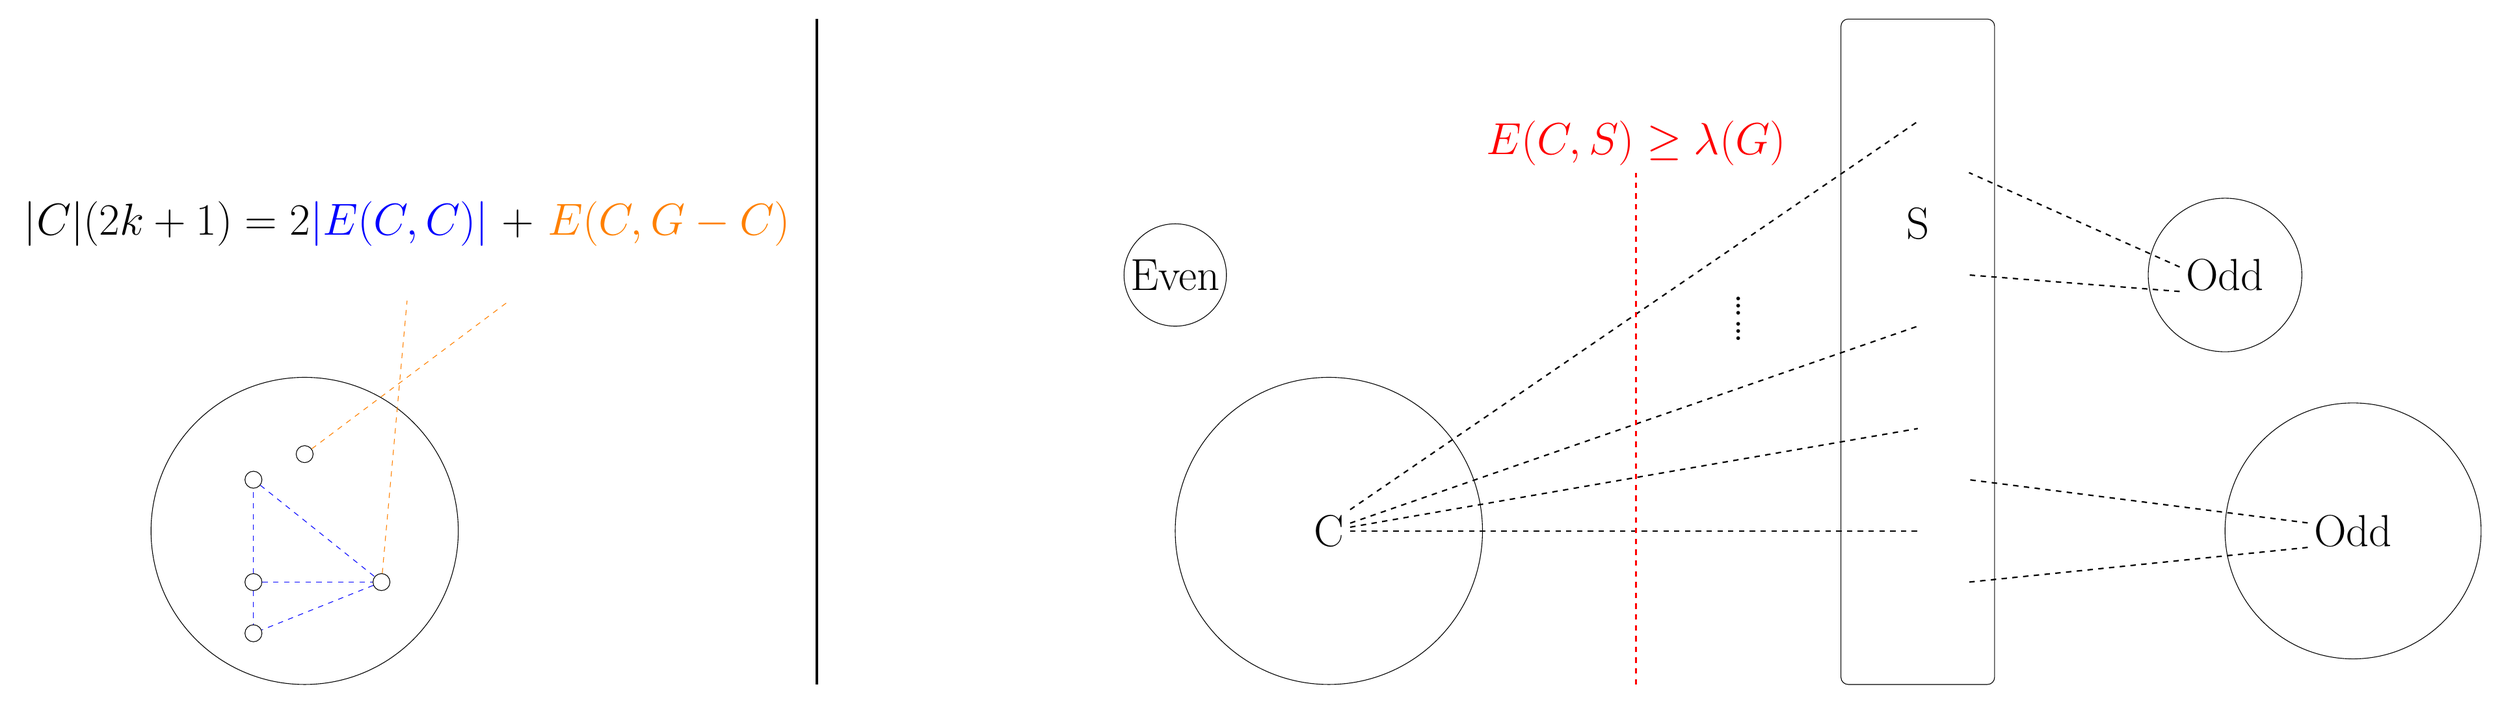
\begin{tikzpicture}
            % LHS Drawing
            \draw (0,0) circle (3cm);
            \node[circle, draw = black] (node-1) at (-1,-1) {};
            \node[circle, draw = black] (node-2) at (-1,1) {};
            \node[circle, draw = black] (node-3) at (1.5,-1) {};
            \node[circle, draw = black] (node-4) at (-1,-2) {};
            \node[circle, draw = black] (node-5) at (0,1.5) {};
            \draw[dashed, blue] (node-1) -- (node-2);
            \draw[dashed, blue] (node-1) -- (node-3);
            \draw[dashed, blue] (node-1) -- (node-4);
            \draw[dashed, blue] (node-2) -- (node-3);
            \draw[dashed, blue] (node-3) -- (node-4);
            \draw[dashed, orange] (node-3) -- (2,4.5);
            \draw[dashed, orange] (node-5) -- (4,4.5);
            \node at (2, 6.0) {\Huge $|C|(2k + 1) = 2$\textcolor{blue}{$|E(C,C)|$} + \textcolor{orange}{$E(C, G-C)$}};

            % Separating Line
            \draw[very thick] (10, -3) -- (10, 10);

            % RHS Drawing
            \draw (20, 0) circle (3cm) node (C) {\Huge C};
            \draw (17, 5) circle (1cm) node {\Huge Even};
            \draw[rounded corners] (30, -3) rectangle (33, 10);
            \node at (31.5, 6) {\Huge S};
            \draw(40, 0) circle (2.5cm) node (N1) {\Huge Odd};
            \draw(37.5, 5) circle (1.5cm) node (N2) {\Huge Odd};
            \draw[dashed, thick] (C.0) -- (31.5, 0);
            \draw[dashed, thick] (C.10) -- (31.5, 2);
            \draw[dashed, thick] (C.20) -- (31.5, 4);
            \draw[dashed, thick] (C.45) -- (31.5, 8);
            \draw[dashed, thick] (N2.200) -- (32.5, 5);
            \draw[dashed, thick] (N2.170) -- (32.5, 7);
            \draw[dashed, thick] (N1.200) -- (32.5, -1);
            \draw[dashed, thick] (N1.170) -- (32.5, 1);
            \node at (28, 4.5) {\Huge $\vdots$};
            \node at (28, 4) {\Huge $\vdots$};
            \draw[very thick, red, dashed] (26, -3) -- (26, 7) node[text=red,anchor=south] {\Huge $E(C, S) \geq \lambda(G)$};
        \end{tikzpicture}
    }
\end{figure}

Moreover, from the previous equality we observe that LHS has the parity of $|C|$, and the RHS has the parity of $|E(C,S)|$. Thus, $|C|$ and $|E(C,S)|$ have the same parity. In particular, $|E(C,S)|$ is odd. Lastly, given that $S$ disconnects $G$, by definition of edge connectivity we have
$$|E(C,S)| \geq \lambda(G) = \lbrace 2k, 2k + 1 \rbrace \overset{|E(C,S)| odd}{\Longrightarrow} |E(C,S)| \geq 2k + 1$$

Inserting this last inequality to (\ref{edge-ineq}) we have:
$$c_o(G-S)(2k + 1) \leq \#\lbrace\text{edges incident to S from odd components}\rbrace \leq |S|(2k + 1) \Rightarrow c_o(G-S) \leq |S|$$
which is exactly Tutte's condition, and hecne $G$ contains a perfect matching.

\subsection[Matchings 3]{Show that the edges of a regular bipartite graph can be decomposed into pairwise disjoint matchings.}

Let $G$ be a $k$-regular bipartite graph, and let $X$ and $Y$ the left and right vertex sets.
Note that $k$-regularity implies $|X| = |Y|$.
Now consider $S \subset X$, $k|S| = |N(S)| \subset Y$.
Let us recall Hall's theorem:
\begin{theorem}[Hall]
    Let $G = (X \cup Y, E)$ be a bipartite graph.
    There is a matching $M$ in $G$ covering all vertices of $X$ if and only if for every $U \subset X$ we have
    $$ |N(U)| \geq |U| $$
\end{theorem}
It is clear that $S > |N(S)|$ implies that there is a vertex with cardinality greater than $k$ (not possible) hence $S \leq N(S)$ and we have a matching (in fact, a perfect one) in $G$.

Let us remove the edges corresponding to this matching, and we have a $k-1$-regular graph.
We progress similarly until we have our edge partition.

\subsection[Matchings 6]{Show that a graph $G$ of order $n$ contains $\frac{n-k}{2}$ independent edges if and only if for every $S \subset V(G)$, it holds that}
$$c_o(G-S) \leq |S| + k$$

Let us consider $S > 0$, otherwise the statement trivially holds.

\begin{remark}
    An independent edge set of a graph $G$ is a subset of the edges such that no two edges in the subset shares a vertex of $G$.
\end{remark}

\begin{itemize}
    \item[$(\Rightarrow)$] We argue by contrapositive.
        $c_o(G-S) > |S| + k$ implies that there are at least $k+1$ more odd components than elements in $S$.
        This in turn means that, at most, we would have an $(n - k -1)$-matching from the odd components to $S$.
    \item[$(\Rightarrow)$] Let us build $G'$ such that $V(G') = V(G) \cup \{v_1, \dots, v_k \}$, we add $k$ new vertices connected to all vertices in $G$.
        Let us now observe that, for all $S' \subset V'$:
        \begin{enumerate}
            \item If $\exists v_i \: | \: v_i \not\in S'$ then $G'$ is connected and $c_o(G' - S') < 1 \leq |S'|$.
            \item If $\{ v_1, \dots, v_k \} \subseteq S' \Rightarrow S' = \{v_1, \dots, v_k \} \cup S$ for some $S$ in $G$.
                Then:
                $$c_o(G' - S') = c_o(G - S) \leq |S| + k = |S'|$$
        \end{enumerate}
        (1) and (2) prove that $G'$ satisfies the Tutte condition, and hence there exists a $n$-matching in $G'$, hence we have an $(n-k)$-matching in $G$ as we wanted to prove.
\end{itemize}

\subsection[Matchings 7]{(i) Show that there is an ordering of the vertices of $G$ such that the greedy coloring algorithm uses only $\chi(G)$ colors. (ii) Find a bipartite graph with $2n$ vertices which admits an ordering for which the greedy coloring algorithm uses $n$ colors. (iii) For each $k$ find a tree $T$ with maximum degree $k$ which admits an ordering for which the greedy coloring algorithm uses $k+1$ colors.}

\subsection[Matchings 8]{Let $G$ be a graph which contains no induced subgraphs isomorphic to $P_4$. Show that the greedy coloring algorithm always uses $\chi(G)$ colors.}
\subsection[Matchings 9]{Show that (i) $\chi(G\square H) = \max\{\chi(G),\chi(H)\}$ and (ii) $\chi(G\times H) = \max\{\chi(G),\chi(H)\}$}

\begin{itemize}
    \item[(i)] Let us first observe that $G, H \subseteq G \square H$ and that $A \subseteq B \Rightarrow \chi(A) \leq chi(B)$.
        Therefore it is clear that $\max\{\chi(G), \chi(H)\} \leq \chi(G \square H)$.

        Secondly, $u$ and $v$ are adjacent in $G \square H$ if they agree on one coordinate and are adjacent in the other one, then $f(u,v) = \chi(u) + \chi(v) \mod \max\{\chi(G), \chi(H)\}$ is a proper coloring.
    \item[(ii)] We know that a graph is $k$-colorable if and only if it has an homomorphism to $K_k$. 
        Observe that $G \times H$ has clear homomorphisms (projections) to $G$ and $H$ and hence it exists an homomorphism $G \times H$ to $K_k$ and $K_g$.
        Thus, the coloring number is the minimum of the two.
\end{itemize}

    \newpage
    \section{Planar Graphs}

\subsection[Planar Graphs 2]{2. Show that a triangulation is $3$-colorable if and only if it is Eulerian (all vertices have an even degree).}

\begin{itemize}
    \item[$(\Rightarrow)$] We will argue by contrapositive:
        $$ G \text{ triangulation not eulerian } \Rightarrow \exists v \in V(G) \text{ s.t. } d(v) \text{ is odd } \Rightarrow \text{ not 3-colorable }$$
    \item[$(\Leftarrow)$] Let us first observe the following:
        $$ G \text{ triangulation } \Rightarrow m = 3n -6$$
        With this, we can see that the minimum degree can't be 6, hence it must be at least 4.
        Let's then pick $v$ such that $d(v) = 4$.
        Draw a romboid with $v$ in the middle and contract one of the diagonals and apply induction.
\end{itemize}


\subsection[Planar Graphs 10]{10. Show that the only non-planar 3-connected graph not containing a subdivision of $K_{3,3}$ is $K_5$.}

\subsection[Planar Graphs 11]{11. Show that a graph is outerplanar ifa nd only if it does not contain a subdivision of $K_4$ or $K_{2,3}$.}

\begin{definition}[Outerplanar Graph]
    A graph $G$ is outerplanar if it admits a plane embedding in which all vertices are in the outer face.
\end{definition}

Given $G = (V, E)$ let $G' = (V \cup \{ x\}, E \cup \{ xy \: | \: y \in V \})$.

\begin{claim}
    $G$ is outerplanar if and only if $G'$ is planar
\end{claim}
\begin{proof}
    \begin{itemize}
        \item[$(\Rightarrow)$] If all vertices are in the outer face, clearly we can connect each one to the center one without crossing.
        \item[$(\Leftarrow)$] Let's suppose $G$ is not outerplanar, then $\exists v$ not in the outer face.
            Then necessarily $\{x , v\}$ produces a crossing and $G'$ is not planar.
    \end{itemize}
\end{proof}

It is clear that we have,
$$ G \text{ outerplanar } \Leftrightarrow G' \text{ planar } \Leftrightarrow G' \text{ does not contain a subdivision of $K_5$ or $K_{3,3}$ }$$
Lastly let us prove the following claim:
\begin{claim}
    $G$ does not contain a subdivision of $K_4$ or $K_{2,3}$ if and only if $G'$ does not contain a subdivision of $K_5$ or $K_{3,3}$.
\end{claim}
\begin{proof}
    \begin{itemize}
        \item[$(\Rightarrow)$] OK
        \item[$(\Leftarrow)$] Suppose that $G$ contains a subdivision of $K_4$ or $K_{2,3}$ then, joining $x$ with all vertices of $G$ we produce either a subdivision of $K_5$ or $K_{3,3}$ within $G'$.
    \end{itemize}
\end{proof}

    \newpage
    \section{Graph Minors 1}

\subsection[Minors 1 - 1]{Prove that every 3-connected graph contains $K_4$ as a minor.}

Let $G = (V,E)$ be a 3-connected graph.
Using Menger's theorem the following claim holds:
\begin{claim}
    A graph $G$ is $k$-connected if and only if for every pair $u,v \in V(G)$ of non-adjacent vertices, there are $k$ internally disjoint ($u-v$)-paths in $G$.
\end{claim}
Let now $u,v \in V(G)$ be two non-adjacent vertices, and $P_1, P_2, P_3$ three internally disjoint $(u-v)$-paths.

Let $S$ be the shortest path between all pair of internal vertices in $P_1$, $P_2$, and $P_3$.
This is, have $S$ join the two closest internal vertices in the disjoint paths.

W.l.o.g. let $p \in V(P_2) \backslash \{u, v \}$ and $q \in V(P_3) \backslash \{ u, v\}$ be the end vertices of $S$.
If $V(S) \cap V(P_1) \neq \emptyset$, take $z \in V(S) \cap V(P_1)$ and taking the subpath $p-z$ or $z-q$ we reach a contradiction with the length of $S$.
Hence we have $V(S) \cap V(P_1) = \emptyset$.
Then $u,v,p,q$ (see supporting drawings) from a subdivision of $K_4$ (topological minor) and therefore $G$ has $K_4$ as a minor.
\begin{figure}[h!]
    \centering
    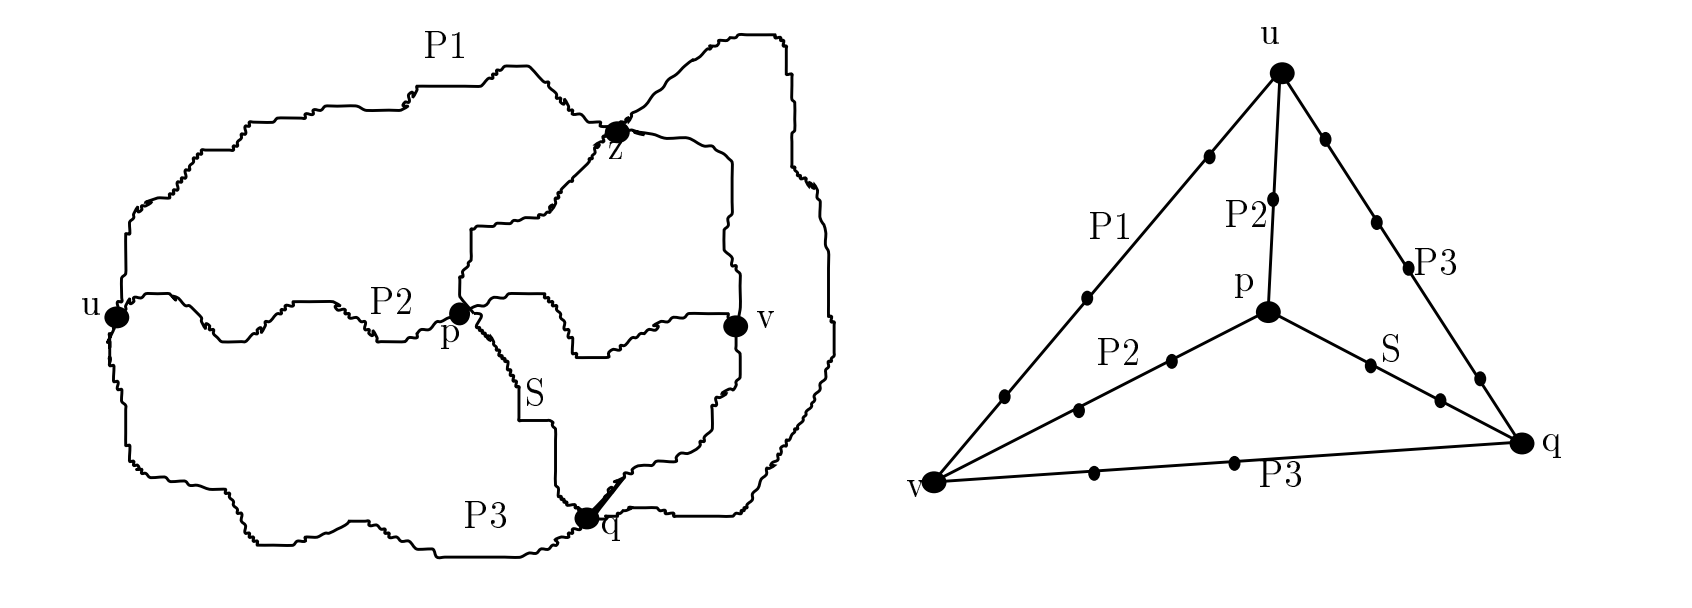
\includegraphics[width=\textwidth]{img/minors_1_1.png}
\end{figure}

\subsection[Minors 1 - 2]{Show that a graph is outerplanar if and only if it does not contain a subdivision of $K_4$ or $K_{2,3}$.}

Done - Problem 11 of Planar Graphs.

\subsection[Minors 1 - 3]{Show that a series-parallel graph with $n$ vertices has at most $2n -3$ edges. Show also that $\chi(G) \leq 3$.}

Let us start off with two definitions:
\begin{definition}[Edge Confluency]
    Two edges $e,f$ are \textbf{confluent} if there are no cycles $C, D$ in $G$ such that $C$ meets $e$ and $f$ in the same direction but $D$ meets them in the opposite.
\end{definition}

\begin{definition}[Series-Parallel Graph]
    A \textbf{series-parallel} graph can be defined either:
    \begin{itemize}
        \item Every pair of edges of $G$ are confluent.
        \item If and only if $G$ does not contain the complete graph $K_4$ as minor: $Forb(K_4)$.
    \end{itemize}
\end{definition}

We will prove the bound on the number of edges by induction on the number of vertices.
\begin{itemize}
    \item \textbf{Case n=3:} at most three edges, $3 \leq 2n - 3 = 1$
    \item \textbf{Inductive case:}
        Note that if $G$ does not contain $K_4$ as a minor and $n \geq 4$, there must exist $v \in V(G)$ such that $d(v) \leq 2$.
        Further, removing a vertex does not induce such a clique.
        Hence,
        $$E(G) \leq E(G \backslash v) + 2 \leq 2 V(G \backslash V) -3 + 2 = 2V(G) -3$$
\end{itemize}

The reason for the chromatic number is similar.
We proceed by induction: remove such vertex, color the graph, and then put it back in and assign one of the three colors.

\subsection[Minors 1 - 5]{Let $H$ be a graph. Show that there is a finite list $H_1, \dots, H_K$ of graphs such that a graph contains $H$ as a minor if and only if contains $H_i$ as a subdivision for some $i$.}

Let us firstly observe the following breakdown:
\begin{itemize}
    \item $\preceq$: can be decomposed in a series of edge contractions and edge deletion (taking subgraphs).
    \item $\preceq_{T}$: can be decomposed in a series of subdivisions and edge deletions.
\end{itemize}
Let us then observe that it suffices to prove that we can obtain H from G through a series of contractions because we could always arrange the intermediate graphs in such a way:
$$H \preceq H_N' \preceq \dots \preceq H_{k+1}' \preceq H_k' \preceq \dots \preceq H_1' \preceq G$$
such that $H_1', \dots, H_k'$ are deletions and $H_{k+1}', \dots, H_N'$ are contractions.
Because it is clear that if $G'$ is obtained from $G$ by deleting some edges, $G' \preceq_T G$.

\begin{definition}[Smoothing]
    Let $v \in V(G)$.
    \textbf{Smoothing:} $G$ at $v$ means replacing $v$ with two new vertices $v_1, v_2$ generating $G'$ such that:
    $$V(G') = V(G)\backslash \{v\} \cup \{v_1, v_2\} \quad E(G') = E(G)\backslash \{ vy \: : \: vy \in E(G) \} \cup \{ v_1y \vee v_2y \: : \: vy \in E(G) \}$$
    Note that smoothing is the inverse operation to contracting edges.
\end{definition}

\begin{definition}[Proper Smoothing]
    Given $v \in V(G)$, $d(v) \geq 4$, a \textbf{proper smoothing} of $G$ at $v$ is a smoothing such that $d(v_1), d(v_2) < d(V)$.
\end{definition}

\begin{definition}[Non-Proper Smoothing]
    Given $v \in V(G)$ if either:
    \begin{enumerate}
        \item We smooth $G$ at $v$ with $d(v) \leq 3$ or
        \item We smooth $G$ at $v$, $d(v) \geq 4$, and either $d(v_1) = d(v)$ or $d(v_2) = d(v)$
    \end{enumerate}
    we call this a \textbf{non-proper smoothing}.
\end{definition}

\begin{claim}
    The edge deletion induced by a non-proper smoothing is equivalent to a subdivision.
\end{claim}

As a consequence we can reduce our study to chains of proper smoothing.

Lastly, for the graph $H$ consider the set of all graphs $F_H$ such that after one contraction, we get $H$ as a minor.
$F_H$ is a finite set.
For each $H_i \in F_H$ consider the set $S_{H_i}$ consisting of all graphs obtained from $H_i$ by \textbf{properly smoothing} $H_i$ at any subset of appropriate vertices.
It remains to show that $F_H \cup (\cup_i S_{H_i}) \: \forall H_i \in F_H$ satisfies the statement.

    \newpage
    \subsection[Minors 2 - 1]{Show that every graph $G$ with treewidth $tw(G) \leq k$ has chromatic number $\chi(G) \leq k$.}

\subsection[Minors 2 - 3]{Let $G$ be a $k$-sum of graphs $G_1$ and $G_2$, $tw(G) \leq \max\{tw(G_1), tw(G_2)\}$.}

\subsection[Minors 2 - 5]{Show that $tw(P_n \square P_n) = n-1$.}

\subsection[Minors 2 - 7]{Is the class of trees well-ordered by the subgraph ordering? Is the class of graphs well-ordered by the topological minor relation?}

    \newpage
    \section{Spectra of Graphs}

\subsection[Spectra -1]{1. Let $H_S$ be the hyperoctahedral graph obtained from the complete graph $K_{2s}$ by removing a perfect matching. Compute the spectrum of $H_2s$.}

The adjacency matrix of a perfect matching with $2s$ vertices can be written as a circulant matrix:
$$\text{circ}(0, \dots, 0, 1, 0, \dots, 0) \quad \text{ 1 at position $s+1$ }$$
just match vertices $1, \dots, s$ to vertices $s + 1, \dots, 2s$.

Hence the Hyperoctahedral graph (complementary of a perfect $2s$-matching has also a circulant adjacency matrix:
$$\text{circ}(0, 1, \dots, 1, 0, 1, \dots, 1) \quad \text{ 0s in position $0$ and $s + 1$ }$$
To compute it's eigenvalues we will use the known property of circulant graphs:
$$\lambda_k = \sum_{j=2}^n a_j \omega^{(j - 1)k} \quad \text{ where } \quad \omega = e^{\frac{2\pi i}{n}}$$

Now let us observe that:
\begin{itemize}
    \item If $k=0$: it is clear that $\lambda_0 = n -2$.
    \item If $k \neq 0$: substitute the coefficients $a_j$, and use that all the unit roots add to 0.
\end{itemize}

\subsection[Spectra - 2]{2. Show that the Petersen graph is the complement of the line graph of $K_5$. Compute the spectrum of the Petersen graph.}

\begin{definition}[Line Graph]
    Given a graph $G$, its line graph $L(G)$ is a graph such that:
    \begin{itemize}
        \item Each vertex of $L(G)$ represents an edge of $G$.
        \item Two vertices in $L(G)$ are adjacent if and only if their respective edges share a common endpoint in $G$.
    \end{itemize}
\end{definition}

Firstly, let us include a picture of the Petersen graph (which has 10 vertices and 15 edges):
\begin{figure}[h!]
    \centering
    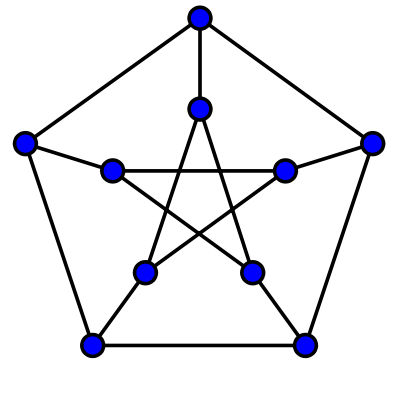
\includegraphics[width=.2\textwidth]{img/spectra_2.png}
\end{figure}

It is clear from the construction that $L(K_5)$ is 6-regular as each edge is incident to two vertices with three different incident edges each.
Further $L(K_5)$ has 10 vertices, and so does it's complementary.
Therefore it is clear that the complementary of the line graph is 3-regular with 10 vertices, hence it is the Petersen graph.

To compute its spectra, we will use the two following lemmas:
\begin{lemma}[Complement of a Graph]
    Let $G$ be an $r$-regular graph. Then,
    $$\phi(\bar{G}, x) = (-1)^n\left( \frac{x + r + 1 - n}{x + r + 1} \right) \phi(G, -x -1)$$
    where $\phi$ denotes the characteristic polynomial. 
\end{lemma}
\begin{lemma}[Line Graphs]
    Let $L(G)$ denote the line graph of $G$. Then if $G$ is $r$-regular,
    $$\phi(L(G), x) = (x + 2)^{m - n} \phi(G, x + 2 -r)$$
\end{lemma}
combining this two lemmas with the spectra of a graph with a circulant adjacency matrix ($K_5$) we can easily check the statement.

\subsection[Spectra - 3]{3. Check that $K_{10}$ contains two edge-disjoint copies of a Petersen graph. Show that $K_10$ does not contain three edge-disjoint copies of the Petersen graph.}

To see that it contains two edge-disjoint copies, it suffices to provide a drawing.
To see that it does not contain a third one, let us recall that the eigenvalues of the Petersen graph are $3$ with a multiplicity of 1, 1 with multiplicity of 5 and -2 with multiplicity of 4.
Let $A$ and $B$ be the adjacency matrix of the two edge-disjoint Petersen graphs, the remaining edge-disjoint graph $C$ would have an adjacency matrix:
$$C = 1_{10 \times 10} - I_{10 \times 10} - A - B$$
there exists $z \in V_A \cap V_B$ such that $z$ is orthogonal to 1, hence we have:
$$C z = (J - I - A - B)z = 0 = 0 - z - Az - Bz = -3z$$
and -3 is an eigenvalue of $C$ hence $C$ can not be a Petersen graph.

\subsection[Spectra - 4]{4. A graph $G$ is strongly regular with parameters $(n, r, \lambda, \mu)$ if it is a $r$-regular graph with $n$ vertices such that every two adjacent (non-adjacent) vertices have exactly $\lambda$ (resp. $\mu$) common neighbours. Show that the spectrum consists on 3 different graphs.}

First of all, the adjacency matrix of a regular graph is a matrix $A$ such that each row and column consists of exactly $r$ ones and $n-r$ zeros.
Then the square of that matrix has:
\begin{itemize}
    \item The main diagonal consisting in $r$'s: the number of walks of length 2 from a vertex to itself is their degree.
    \item Each row has $r$ $\lambda$s: the number of walks of length 2 between two adjacent vertices is, by definition, $\lambda$.
    \item The rest of the elements are $\mu$s.
\end{itemize}
Hence it can be expressed in the following way:
$$A^2 = rI + \lambda A + \mu(1_{n \times n} - I - A) = A^2 - (\lambda - \mu)A - (r - \mu)I - \mu V = 0$$
hence if $x$ is an eigenvalue of $A$, it must satisfy:
$$x^2 - (\lambda - \mu)x - (r - \mu) = 0$$

\subsection[Spectra - 5]{5. Let $G$ be a bipartite graph. (i) Show that the spectrum of $G$ is symmetric. (ii) Compute the spectrum of the bipartite complete graph $K_{r,s}$.}

\end{document}
